\documentclass{article}
\usepackage[margin=1in]{geometry}
\usepackage[linesnumbered,ruled,vlined]{algorithm2e}
\usepackage{amsfonts}
\usepackage{amsmath}
\usepackage{amssymb}
\usepackage{amsthm}
\usepackage{enumitem}
\usepackage{fancyhdr}
\usepackage{hyperref}
\usepackage{minted}
\usepackage{multicol}
\usepackage{pdfpages}
\usepackage{standalone}
\usepackage[many]{tcolorbox}
\usepackage{tikz-cd}
\usepackage{transparent}
\usepackage{xcolor}
% \tcbuselibrary{minted}

\author{Nathan Solomon}

\newcommand{\fig}[1]{
    \begin{center}
        \includegraphics[width=\textwidth]{#1}
    \end{center}
}

% Math commands
\renewcommand{\d}{\mathrm{d}}
\DeclareMathOperator{\id}{id}
\DeclareMathOperator{\im}{im}
\DeclareMathOperator{\proj}{proj}
\DeclareMathOperator{\Span}{span}
\DeclareMathOperator{\Tr}{Tr}
\DeclareMathOperator{\tr}{tr}
\DeclareMathOperator{\ad}{ad}
\DeclareMathOperator{\ord}{ord}
%%%%%%%%%%%%%%% \DeclareMathOperator{\sgn}{sgn}
\DeclareMathOperator{\Aut}{Aut}
\DeclareMathOperator{\Inn}{Inn}
\DeclareMathOperator{\Out}{Out}
\DeclareMathOperator{\stab}{stab}

\newcommand{\N}{\ensuremath{\mathbb{N}}}
\newcommand{\Z}{\ensuremath{\mathbb{Z}}}
\newcommand{\Q}{\ensuremath{\mathbb{Q}}}
\newcommand{\R}{\ensuremath{\mathbb{R}}}
\newcommand{\C}{\ensuremath{\mathbb{C}}}
\renewcommand{\H}{\ensuremath{\mathbb{H}}}
\newcommand{\F}{\ensuremath{\mathbb{F}}}

\newcommand{\E}{\ensuremath{\mathbb{E}}}
\renewcommand{\P}{\ensuremath{\mathbb{P}}}

\newcommand{\es}{\ensuremath{\varnothing}}
\newcommand{\inv}{\ensuremath{^{-1}}}
\newcommand{\eps}{\ensuremath{\varepsilon}}
\newcommand{\del}{\ensuremath{\partial}}
\renewcommand{\a}{\ensuremath{\alpha}}

\newcommand{\abs}[1]{\ensuremath{\left\lvert #1 \right\rvert}}
\newcommand{\norm}[1]{\ensuremath{\left\lVert #1\right\rVert}}
\newcommand{\mean}[1]{\ensuremath{\left\langle #1 \right\rangle}}
\newcommand{\floor}[1]{\ensuremath{\left\lfloor #1 \right\rfloor}}
\newcommand{\ceil}[1]{\ensuremath{\left\lceil #1 \right\rceil}}
\newcommand{\bra}[1]{\ensuremath{\left\langle #1 \right\rvert}}
\newcommand{\ket}[1]{\ensuremath{\left\lvert #1 \right\rangle}}
\newcommand{\braket}[2]{\ensuremath{\left.\left\langle #1\right\vert #2 \right\rangle}}

\newcommand{\catname}[1]{{\normalfont\textbf{#1}}}

\newcommand{\up}{\ensuremath{\uparrow}}
\newcommand{\down}{\ensuremath{\downarrow}}

% Custom environments
\newtheorem{thm}{Theorem}[section]

\definecolor{probBackgroundColor}{RGB}{250,240,240}
\definecolor{probAccentColor}{RGB}{140,40,0}
\newenvironment{prob}{
    \stepcounter{thm}
    \begin{tcolorbox}[
        boxrule=1pt,
        sharp corners,
        colback=probBackgroundColor,
        colframe=probAccentColor,
        borderline west={4pt}{0pt}{probAccentColor},
        breakable
    ]
    \color{probAccentColor}\textbf{Problem \thethm.} \color{black}
} {
    \end{tcolorbox}
}

\definecolor{exampleBackgroundColor}{RGB}{212,232,246}
\newenvironment{example}{
    \stepcounter{thm}
    \begin{tcolorbox}[
      boxrule=1pt,
      sharp corners,
      colback=exampleBackgroundColor,
      breakable
    ]
    \textbf{Example \thethm.}
} {
    \end{tcolorbox}
}

\definecolor{propBackgroundColor}{RGB}{255,245,220}
\definecolor{propAccentColor}{RGB}{150,100,0}
\newenvironment{prop}{
    \stepcounter{thm}
    \begin{tcolorbox}[
        boxrule=1pt,
        sharp corners,
        colback=propBackgroundColor,
        colframe=propAccentColor,
        breakable
    ]
    \color{propAccentColor}\textbf{Proposition \thethm. }\color{black}
} {
    \end{tcolorbox}
}

\definecolor{thmBackgroundColor}{RGB}{235,225,245}
\definecolor{thmAccentColor}{RGB}{50,0,100}
\renewenvironment{thm}{
    \stepcounter{thm}
    \begin{tcolorbox}[
        boxrule=1pt,
        sharp corners,
        colback=thmBackgroundColor,
        colframe=thmAccentColor,
        breakable
    ]
    \color{thmAccentColor}\textbf{Theorem \thethm. }\color{black}
} {
    \end{tcolorbox}
}

\definecolor{corBackgroundColor}{RGB}{240,250,250}
\definecolor{corAccentColor}{RGB}{50,100,100}
\newenvironment{cor}{
    \stepcounter{thm}
    \begin{tcolorbox}[
        enhanced,
        boxrule=0pt,
        frame hidden,
        sharp corners,
        colback=corBackgroundColor,
        borderline west={4pt}{0pt}{corAccentColor},
        breakable
    ]
    \color{corAccentColor}\textbf{Corollary \thethm. }\color{black}
} {
    \end{tcolorbox}
}

\definecolor{lemBackgroundColor}{RGB}{255,245,235}
\definecolor{lemAccentColor}{RGB}{250,125,0}
\newenvironment{lem}{
    \stepcounter{thm}
    \begin{tcolorbox}[
        enhanced,
        boxrule=0pt,
        frame hidden,
        sharp corners,
        colback=lemBackgroundColor,
        borderline west={4pt}{0pt}{lemAccentColor},
        breakable
    ]
    \color{lemAccentColor}\textbf{Lemma \thethm. }\color{black}
} {
    \end{tcolorbox}
}

\definecolor{proofBackgroundColor}{RGB}{255,255,255}
\definecolor{proofAccentColor}{RGB}{80,80,80}
\renewenvironment{proof}{
    \begin{tcolorbox}[
        enhanced,
        boxrule=1pt,
        sharp corners,
        colback=proofBackgroundColor,
        colframe=proofAccentColor,
        borderline west={4pt}{0pt}{proofAccentColor},
        breakable
    ]
    \color{proofAccentColor}\emph{\textbf{Proof. }}\color{black}
} {
    \qed \end{tcolorbox}
}

\definecolor{noteBackgroundColor}{RGB}{240,250,240}
\definecolor{noteAccentColor}{RGB}{30,130,30}
\newenvironment{note}{
    \begin{tcolorbox}[
        enhanced,
        boxrule=0pt,
        frame hidden,
        sharp corners,
        colback=noteBackgroundColor,
        borderline west={4pt}{0pt}{noteAccentColor},
        breakable
    ]
    \color{noteAccentColor}\textbf{Note. }\color{black}
} {
    \end{tcolorbox}
}


\fancyhf{}
\setlength{\headheight}{24pt}

\date{\today}
\title{Physics 127 Homework \#1}

\begin{document}
\maketitle

\begin{prob}
\end{prob}
\begin{enumerate}[label=(\alph*)]
    \item The ``square matrix $g$" is actually $g_\nu^\mu$, and the transpose of $v^\mu$ is $v_\mu$. So including the indices, $v \cdot w$ can be written as
        \[ v \cdot w = v^T g w = v^\mu g_{\mu \nu} w^\nu. \]
        This is symmetric because
        \[ w \cdot v = w^\mu g_{\mu \nu} v^\nu = w^\nu g_{\nu \mu} v^\mu = v^\mu g_{\nu \mu} w^\nu = v^\mu g_{\mu \nu} w^\nu = v \cdot w. \]
        Note that I used the fact that $g_{\nu \mu} = g_{\mu \nu}$, which is valid because both sides are equal to
        \[ g_{\mu \nu} = e_0 \otimes e_0 - e_1 \otimes e_1 - e_2 \otimes e_2 - e_3 \otimes e_3 = g_{\nu \mu}. \]
        If $v=w=x$, then
        \[ x \cdot x = x_0x^0 - x_1x^1 - x_2x^2 - x_3x^3. \]
    \item Let
        \[ \mathcal{B} = \left\{ e^0, e^1, e^2, e^3 \right\} \]
        be a basis for $\R^4$, and for each basis vector $e^\mu$, denote the dual basis vector as $(e^*)^\mu = e_\mu$. Then $\Lambda_\nu^\mu$ is a linear combination of terms of the form $e_\nu^\mu := e_\nu \otimes e^\mu$. The transpose of that is $(e^T)_\nu \otimes (e^T)^\mu = e^\nu \otimes e_\mu = e_\mu^\nu$.
        \par
        Since we have $(e_\nu^\mu)^T = e_\mu^\nu$ for any basis element $e_\nu^\mu$ of $(\R^4)^* \otimes \R^4$, the equation
        \[ (\Lambda^T)_\nu^\mu = \Lambda_\mu^\nu \]
        is true for any $\Lambda: \R^4 \rightarrow \R^4$.
        \par
        The condition for $\Lambda$ to be a Lorentz transformation can be written as
        \[ \Lambda_\rho^\mu g_{\mu \nu} \Lambda_\sigma^\nu = g_{\rho \sigma}, \]
        since matrix multiplication commutes in Einstein notation. If we want to write $g_{\mu \nu}$ as a square matrix, then that equation becomes
        \[ \Lambda_\mu^\rho g_\nu^\mu \Lambda_\sigma^\nu = g_\sigma^\rho, \]
        which is equivalent to $\Lambda^T g \lambda = g$, where $\Lambda$ and $g$ wihtout indices denote type (1, 1) tensors (aka square matrices).
    \item \begin{align*}
            v' \cdot w' &= (\Lambda v) \cdot (\Lambda w) \\
                        &= (\Lambda v)^T g (\Lambda w) \\
                        &= v^T (\Lambda^T g \Lambda) w \\
                        &= v^T g w \\
                        &= v \cdot w.
    \end{align*}
\end{enumerate}

\bigskip
\par
\begin{prob}
\end{prob}
\begin{enumerate}[label=(\alph*)]
    \item \begin{align*}
            \Lambda^T g \Lambda &= \begin{bmatrix}
                \cosh \alpha & \sinh \alpha & 0 & 0 \\
                \sinh \alpha & \cosh \alpha & 0 & 0 \\
                0 & 0 & 1 & 0 \\
                0 & 0 & 0 & 1
            \end{bmatrix} \begin{bmatrix}
                1 & 0 & 0 & 0 \\
                0 & -1 & 0 & 0 \\
                0 & 0 & -1 & 0 \\
                0 & 0 & 0 & -1
            \end{bmatrix} \begin{bmatrix}
                \cosh \alpha & \sinh \alpha & 0 & 0 \\
                \sinh \alpha & \cosh \alpha & 0 & 0 \\
                0 & 0 & 1 & 0 \\
                0 & 0 & 0 & 1
            \end{bmatrix} \\
            &= \begin{bmatrix}
                \cosh \alpha & -\sinh \alpha & 0 & 0 \\
                \sinh \alpha & -\cosh \alpha & 0 & 0 \\
                0 & 0 & -1 & 0 \\
                0 & 0 & 0 & -1
            \end{bmatrix} \begin{bmatrix}
                \cosh \alpha & \sinh \alpha & 0 & 0 \\
                \sinh \alpha & \cosh \alpha & 0 & 0 \\
                0 & 0 & 1 & 0 \\
                0 & 0 & 0 & 1
            \end{bmatrix} \\
            &= \begin{bmatrix}
                \cosh^2 \alpha - \sinh^2 \alpha & 0 & 0 & 0 \\
                0 & \sinh^2 \alpha - \cosh^2 \alpha & 0 & 0 \\
                0 & 0 & -1 & 0 \\
                0 & 0 & 0 & -1
            \end{bmatrix} \\
            &= g. \\
            R^T g R &= \begin{bmatrix}
                1 & 0 & 0 & 0 \\
                0 & 1 & 0 & 0 \\
                0 & 0 & \cos \theta & -\sin \theta \\
                0 & 0 & \sin \theta & \cos \theta
            \end{bmatrix} \begin{bmatrix}
                1 & 0 & 0 & 0 \\
                0 & -1 & 0 & 0 \\
                0 & 0 & -1 & 0 \\
                0 & 0 & 0 & -1
            \end{bmatrix} \begin{bmatrix}
                1 & 0 & 0 & 0 \\
                0 & 1 & 0 & 0 \\
                0 & 0 & \cos \theta & \sin \theta \\
                0 & 0 & -\sin \theta & \cos \theta
            \end{bmatrix} \\
            &= \begin{bmatrix}
                1 & 0 & 0 & 0 \\
                0 & -1 & 0 & 0 \\
                0 & 0 & -\cos \theta & \sin \theta \\
                0 & 0 & -\sin \theta & -\cos \theta
            \end{bmatrix} \begin{bmatrix}
                1 & 0 & 0 & 0 \\
                0 & 1 & 0 & 0 \\
                0 & 0 & \cos \theta & \sin \theta \\
                0 & 0 & -\sin \theta & \cos \theta
            \end{bmatrix} \\
            &= \begin{bmatrix}
                1 & 0 & 0 & 0 \\
                0 & -1 & 0 & 0 \\
                0 & 0 & -\cos^2 \theta - \sin^2 \theta & 0 \\
                0 & 0 & 0 & -\sin^2 \theta - \cos^2 \theta
            \end{bmatrix} \\
            &= g. \\
    \end{align*}
\item $R(\theta)$ is a rotation of the $yz$-plane about the $x$-axis by an angle $\theta$, so $R(\phi)$ is an inverse of $R(\theta)$ iff $\phi+\theta$ is an integer multiple of $2 \pi$. Also, given a rotation matrix $R(\theta)$, you can take the transpose to get $R(\theta)^{-1}$, since $R(\theta)$ is an orthogonal matrix.
    \par
    To take the inverse of a block-diagonal matrix, you can just take the inverse of each block, so the inverse of $\Lambda(\alpha)$ is \begin{align*}
        \Lambda(\alpha)^{-1} &= \begin{pmatrix}
            \begin{bmatrix}
                \cosh \alpha & \sinh \alpha \\
                \sinh \alpha & \cosh \alpha
            \end{bmatrix}^{-1} & 0_{2 \times 2} \\
            0_{2 \times 2} & 1_{2 \times 2}^{-1}
        \end{pmatrix} \\
                             &= \begin{pmatrix}
                                 \begin{bmatrix}
                                     \cosh \alpha & -\sinh \alpha \\
                                     -\sinh \alpha & \cosh \alpha
                                 \end{bmatrix} & 0_{2 \times 2} \\
                                 0_{2 \times 2} & 1_{2 \times 2}
                             \end{pmatrix} \\
                             &= \begin{pmatrix}
                                 \cosh(\alpha) & \sinh(-\alpha) & 0 & 0 \\
                                 \sinh(-\alpha) & \cosh(\alpha) & 0 & 0 \\
                                 0 & 0 & 1 & 0 \\
                                 0 & 0 & 0 & 1
                             \end{pmatrix} \\
                             &= \Lambda(-\alpha).
    \end{align*}
    In conclusion, $R(\theta)^{-1}=R(-\theta)$ and $\Lambda(\alpha)^{-1}=\Lambda(-\alpha)$.
\item \begin{align*}
        \Lambda(\alpha_1) \Lambda(\alpha_2) &= \begin{bmatrix}
            \cosh \alpha_1 & \sinh \alpha_1 & 0 & 0 \\
            \sinh \alpha_1 & \cosh \alpha_1 & 0 & 0 \\
            0 & 0 & 1 & 0 \\
            0 & 0 & 0 & 1
        \end{bmatrix} \begin{bmatrix}
            \cosh \alpha_2 & \sinh \alpha_2 & 0 & 0 \\
            \sinh \alpha_2 & \cosh \alpha_2 & 0 & 0 \\
            0 & 0 & 1 & 0 \\
            0 & 0 & 0 & 1
        \end{bmatrix} \\
                                            &= \begin{bmatrix}
                                                \cosh \alpha_1 \cosh \alpha_2 + \sinh \alpha_1 \sinh \alpha_2 & \cosh \alpha_1 \sinh \alpha_2 + \sinh \alpha_1 \cosh \alpha_2 & 0 & 0 \\
                                                \sinh \alpha_1 \cosh \alpha_2 + \cosh \alpha_1 \sinh \alpha_2 & \sinh \alpha_1 \sinh \alpha_2 + \cosh \alpha_1 \cosh \alpha_2 & 0 & 0 \\
            0 & 0 & 1 & 0 \\
            0 & 0 & 0 & 1
                                            \end{bmatrix} \\
                                            &= \begin{bmatrix}
                                                \cosh(\alpha_1 + \alpha_2) & \sinh(\alpha_1 + \alpha_2) & 0 & 0 \\
                                                \sinh(\alpha_1 + \alpha_2) & \cosh(\alpha_1 + \alpha_2) & 0 & 0 \\
                                                0 & 0 & 1 & 0 \\
                                                0 & 0 & 0 & 1
                                            \end{bmatrix} \\
                                            &= \Lambda(\alpha_1 + \alpha_2). \\
            R(\theta_1) R(\theta_2) &= \begin{bmatrix}
                1 & 0 & 0 & 0 \\
                0 & 1 & 0 & 0 \\
                0 & 0 & \cos \theta_1 & \sin \theta_1 \\
                0 & 0 & -\sin \theta_1 & \cos \theta_1
            \end{bmatrix} \begin{bmatrix}
                1 & 0 & 0 & 0 \\
                0 & 1 & 0 & 0 \\
                0 & 0 & \cos \theta_2 & \sin \theta_2 \\
                0 & 0 & -\sin \theta_2 & \cos \theta_2
            \end{bmatrix} \\
            &= \begin{bmatrix}
                1 & 0 & 0 & 0 \\
                0 & 1 & 0 & 0 \\
                0 & 0 & \cos \theta_1 \cos \theta_2 - \sin \theta_1 \sin \theta_2 & \cos \theta_1 \sin \theta_2 + \sin \theta_1 \cos \theta_2 \\
                0 & 0 & -\sin \theta_1 \cos \theta_2 - \cos \theta_1 \sin \theta_2 & - \sin \theta_1 \sin \theta_2 + \cos \theta_1 \cos \theta_2 \\
            \end{bmatrix} \\
            &= \begin{bmatrix}
                1 & 0 & 0 & 0 \\
                0 & 1 & 0 & 0 \\
                0 & 0 & \cos(\theta_1 + \theta_2) & \sin(\theta_1 + \theta_2) \\
                0 & 0 & -\sin(\theta_1 + \theta_2) & \cos(\theta_1 + \theta_2) \\
            \end{bmatrix} \\
            &= R(\theta_1 + \theta_2).
\end{align*}
\end{enumerate}

\bigskip
\par
\begin{prob}
\end{prob}
For simplicity, I'll ignore the $x^2$ and $x^3$ coordinates, so the point is $x^\mu = (t, x)$, and a Lorentz boost has the form
\[ \Lambda_\mu^\nu = \begin{bmatrix}
    \gamma & \gamma v \\
    \gamma v & \gamma
\end{bmatrix}. \]
If $x^\mu$ is timelike, then $\abs{t}>\abs{x}$, so if you let $v = -x/t$, then $v$ is a valid speed (that is, $\abs{v}<c$), and the boosted event is
\[ y^\nu = \Lambda_\mu^\nu x^\mu = \begin{bmatrix}
    \gamma & -\gamma x / t \\
    -\gamma x / t & \gamma
\end{bmatrix} \begin{bmatrix}
    t \\
    x
\end{bmatrix} = \begin{bmatrix}
    \gamma (t-x^2/t) \\
    0
\end{bmatrix}, \]
which has a spatial coordinate of zero.
\par
Similarly, if $x^\mu$ is spacelike, then $\abs{t}<\abs{x}$, so $v = -t/x$ is a valid speed, and the boosted event is
\[ y^\nu = \Lambda_\mu^\nu x^\mu = \begin{bmatrix}
    \gamma & -\gamma t / x \\
    -\gamma t / x & \gamma
\end{bmatrix} \begin{bmatrix}
    t \\
    x
\end{bmatrix} = \begin{bmatrix}
    0 \\
    \gamma (x - t^2/x)
\end{bmatrix}, \]
whose time coordinate is equal to zero.


\bigskip
\par
\begin{prob}
\end{prob}
The Lorentz group in 3+1 dimensions, $O(1,3)$, is a 6-dimensional Lie group with 4 connected components.
\par
In 2+1 dimensions, the Lorentz group $O(1,2)$ still has 4 connected components, because there is one component which contains the identity matrix, another for which time is reversed (proper \& nonorthochronous), another for which the parity of space is reversed (improper \& orthochronous), and another for which the parities of time and space are both reversed (improper \& nonorthochronous). Those four components are all disconnected because there is no continuous way to interpolate between them. Some representative elements for the respective components are
\[ \begin{bmatrix}
    1 & 0 & 0 \\
    0 & 1 & 0 \\
    0 & 0 & 1
\end{bmatrix}, \begin{bmatrix}
    -1 & 0 & 0 \\
    0 & 1 & 0 \\
    0 & 0 & 1
\end{bmatrix}, \begin{bmatrix}
    1 & 0 & 0 \\
    0 & -1 & 0 \\
    0 & 0 & 1
\end{bmatrix}, \begin{bmatrix}
    -1 & 0 & 0 \\
    0 & -1 & 0 \\
    0 & 0 & 1
\end{bmatrix}. \]
Note that to change the parity of space, we negate 1 of the spatial coordinates, because negating both spatial coordinates would be a proper transformation.
\par
The dimension of each component is 3, because the identity component is generated by the three following types of boosts:
\[ \begin{bmatrix}
    \gamma & \gamma v & 0 \\
    \gamma v & \gamma & 0 \\
    0 & 0 & 1
\end{bmatrix}, \begin{bmatrix}
    \gamma & 0 & \gamma u \\
    0 & 1 & 0 \\
    \gamma u & 0 & \gamma
\end{bmatrix}, \begin{bmatrix}
    1 & 0 & 0 \\
    0 & a & 1-a^2 \\
    0 & a^2-1 & a
\end{bmatrix}, \]
where $v, u, a \in \R$ and $\abs{a}\leq 1$.

\bigskip
\par
\begin{prob}
Alice and Bob both travel from spacetime point $a$ to spacetime point $b$. Alice goes by the straight line path (in Minkowski space); Bob wanders around -- his world line is curved.
\par
Which trip takes longer, according to each traveler’s own watch?
\end{prob}
The answer to this question doesn't change if we Lorentz boost the the frame where $a = (0, 0, 0, 0)$ and $b = (T, 0, 0, 0)$. This is Alice's frame, so she measures her own trip to take time $T$. If Bob's trip is parameterized by $x^\mu(t)$, where $t$ goes from $0$ to $T$, then he measures the duration of his own trip to be
\[ \int_{t=0}^{t=T} \sqrt{ \left( \frac{\partial x^0}{\partial t} \right)^2 - \left( \frac{\partial x^1}{\partial t} \right)^2} \d t. \]
But since the integrand is always positive, it's $\leq 1$ everywhere, and $<1$ somewhere, that integral must work out to be less than $T$.
\par
Therefore, the duration Alice measures for her own trip ($T$) is greater than the duration Bob measures for his own trip.

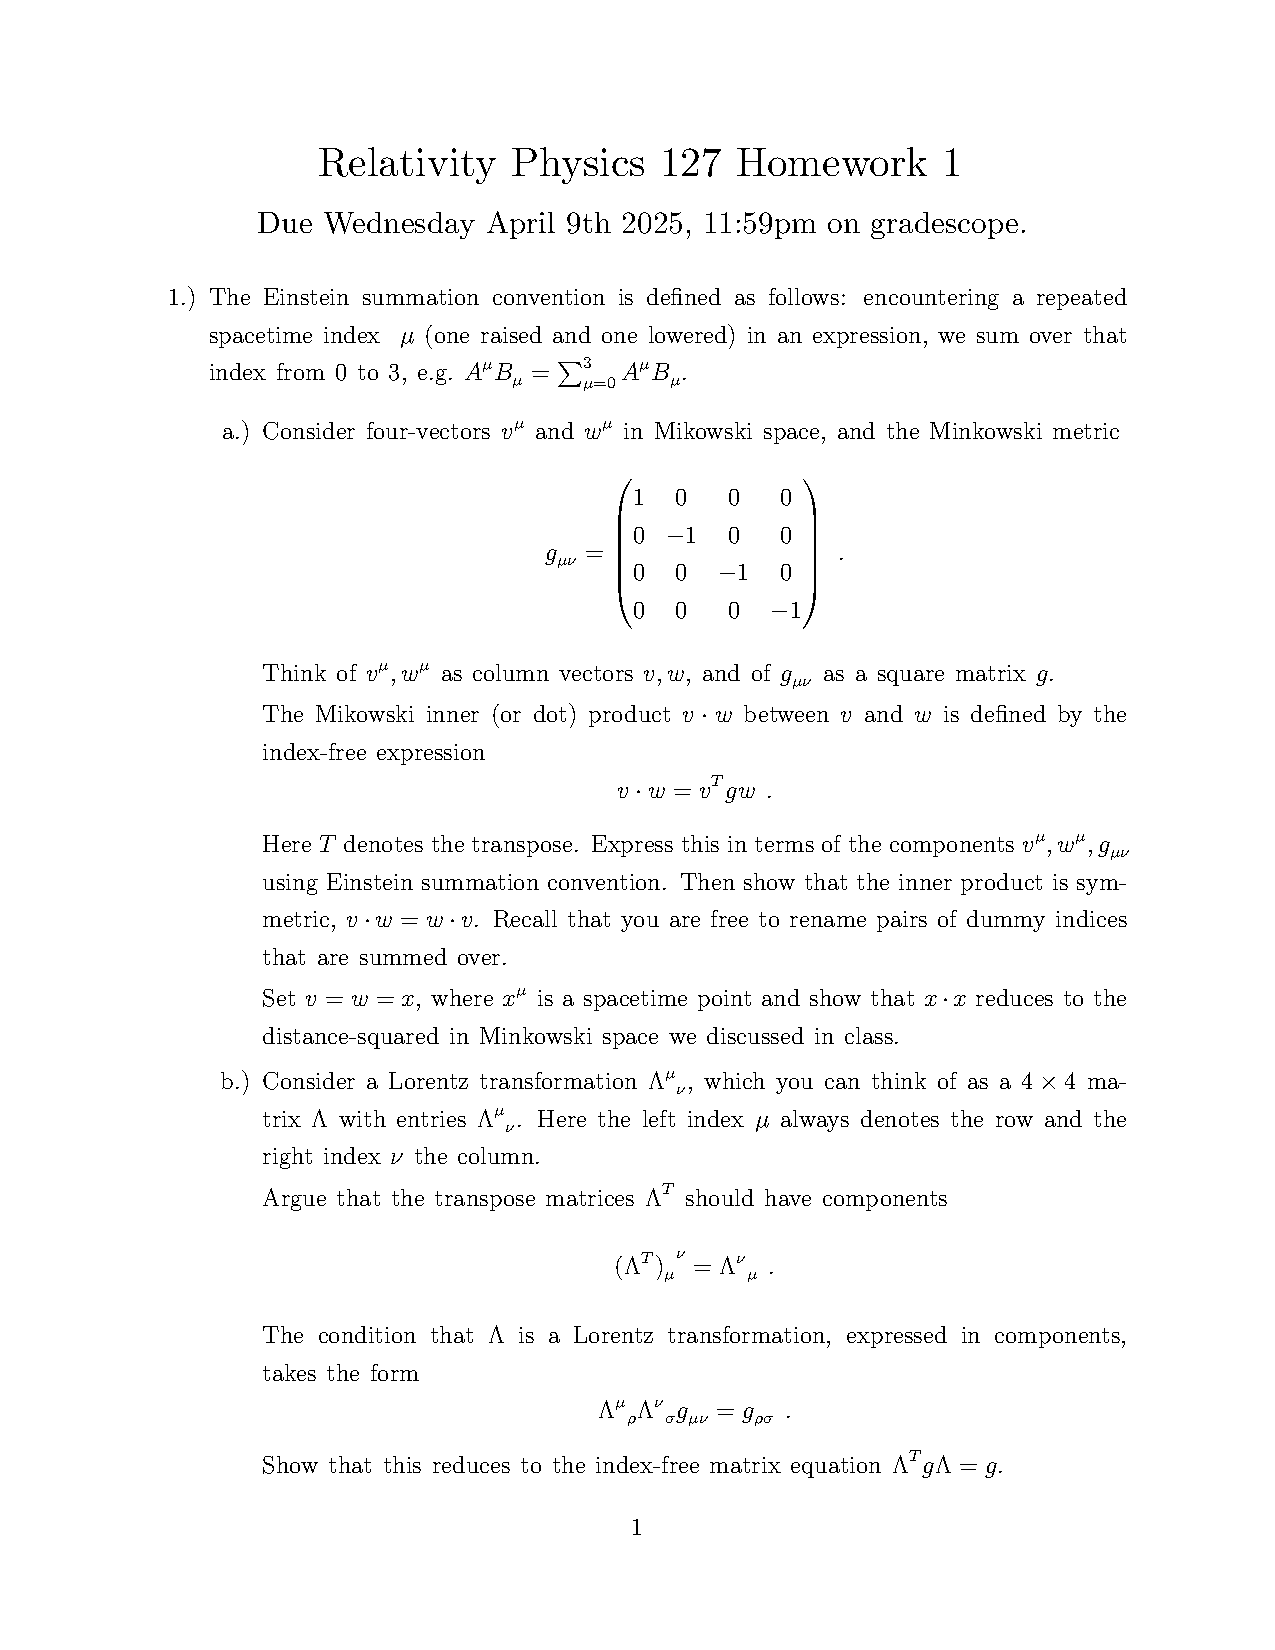
\includepdf[pages=-]{assignment.pdf}

\end{document}
